\chapter{Fibonacci Heaps}

In the previous chapter, union-find postponed work lazily until queries required it. We can push this principle of lazy postponement into priority queues. You have met binary heaps back in Chapter~6: a heap lives in
an array, it keeps the smallest (or largest) thing on top, and it lets you insert
and extract-min in $O(\log n)$ time. For most problems that is plenty.

Some graph algorithms, however, have a heavily skewed workload: they call
one priority-queue operation \emph{thousands} of times for every call to another.
When that happens, we want to make the frequent operation cheaper even if a rarer
operation has to do more cleanup later. That is the exact trade-off a \emph{Fibonacci heap}
is designed for. It is the data structure you reach
for when you want \lstinline|decrease-key| to be, on average, nearly free.

This chapter feels different from the binary-heap chapter. There, the
structure was rigid and the analysis was direct. Here, the structure is loose,
almost messy, and all the cleverness sits in the \emph{amortized} analysis. We
will go slowly. By the end you will understand both the mechanics of each operation
and the structural reasons why the looseness is the point, including why Fibonacci
numbers govern the tree sizes.

\begin{focusbox}
The whole chapter is one trade. We let the heap get structurally lazy and messy
so that \lstinline|insert| and \lstinline|decrease-key| can finish in $O(1)$
amortized time. We pay for that laziness later, all at once, during
\lstinline|extract-min|, which does a big cleanup. Hold onto that image: cheap
deposits now, one expensive cleanup later.
\end{focusbox}

\section{What problem are we actually solving?}
\label{ch20:problem}

Let us start with the customer, not the product. Who needs a fancier heap?

Think about Dijkstra's shortest-path algorithm, or Prim's minimum-spanning-tree
algorithm (we will meet both properly in Chapters~23 and~24; for now just trust the
shape of their work). Both algorithms keep a priority queue of vertices keyed by a
tentative distance. The main loop does this:

\begin{itemize}
  \item Pull out the closest unfinished vertex. That is one \lstinline|extract-min|.
  \item For each edge leaving that vertex, maybe \emph{lower} the key of the
        neighbor on the other end, because we just found a shorter way to reach it.
        That is a \lstinline|decrease-key|.
\end{itemize}

Now count. Over the whole run of the algorithm on a graph with $V$ vertices and
$E$ edges, you do at most $V$ extract-mins (one per vertex) but up to $E$
decrease-keys (one per edge, in the worst case). In a dense graph, $E$ can be as
large as $V^2$. So decrease-key is the operation that gets hammered, and
extract-min is comparatively rare.

\begin{intuitionbox}
A binary heap charges $O(\log n)$ for \emph{both} extract-min and decrease-key.
Dijkstra then costs $O((V+E)\log V)$. The $E\log V$ term dominates, and it is
entirely the fault of decrease-key being logarithmic.

A Fibonacci heap charges $O(\log V)$ \emph{amortized} for extract-min but only
$O(1)$ \emph{amortized} for decrease-key. Now Dijkstra costs
$O(V\log V + E)$. We traded a $\log$ factor off the busiest operation. On dense
graphs that is the difference between $V^2 \log V$ and $V^2$ work for the
relaxation step.
\end{intuitionbox}

So the target is set in stone before we design anything:

\begin{focusbox}
We want a \emph{mergeable} priority queue where:
\begin{center}
\begin{tabular}{lll}
\toprule
operation & we will achieve & (binary heap was) \\
\midrule
\lstinline|insert|        & $O(1)$ amortized & $O(\log n)$ \\
\lstinline|minimum|       & $O(1)$ worst case & $O(1)$ \\
\lstinline|extract-min|   & $O(\log n)$ amortized & $O(\log n)$ \\
\lstinline|decrease-key|  & $O(1)$ amortized & $O(\log n)$ \\
\lstinline|union|         & $O(1)$ worst case & $O(n)$ \\
\bottomrule
\end{tabular}
\end{center}
\end{focusbox}

That \lstinline|union| row deserves a word. ``Mergeable'' means you can take two
whole heaps and splice them into one. With an array-based binary heap that is
expensive --- you essentially rebuild. Fibonacci heaps make it trivial, and that
trivial-merge ability is the seed from which everything else grows.

\section{The idea: lazy bags of trees}

\subsection{From one tree to a forest}

A binary heap is a single tree, kept perfectly balanced inside an array. The
balance is what makes it $O(\log n)$ --- but maintaining balance is also what
makes every operation \emph{pay} that $O(\log n)$.

A Fibonacci heap drops that strict balance requirement. Instead of one carefully shaped
tree, it keeps a \emph{collection} of heap-ordered trees. ``Heap-ordered'' means
the same local rule you already know: in every tree, each node's key is $\le$ the
keys of its children. So the minimum of any one tree is at that tree's root. The
minimum of the \emph{whole} heap is therefore the smallest root among all the
trees --- and we keep a pointer straight to it.

\begin{intuitionbox}
Picture a tabletop covered with little trees, each one a heap. The roots are laid
out in a circle (a doubly linked list joined at the ends), so you can walk from any
root to the next. One special pointer, $\mathit{min}$, always aims at the smallest
root. That is a Fibonacci heap: a circle of root-tops, with $\mathit{min}$ pointing
at the lowest.
\end{intuitionbox}

Here is a small forest. Each tree is heap-ordered, and $\mathit{min}$ points at the
overall smallest root, $3$.

\begin{center}
\begin{tikzpicture}[
  every node/.style={circle,draw,minimum size=6mm,inner sep=1pt,font=\small},
  level distance=9mm, sibling distance=10mm,
  edge from parent/.style={draw,gray}]
  % root list across the top
  \node (r1) at (0,0) {7};
  \node (r2) at (2.2,0) {3};
  \node (r3) at (5.0,0) {18};
  \node (r4) at (6.5,0) {52};

  % min pointer
  \node[draw=none,fill=none,font=\footnotesize\bfseries,structurepurple] at (2.2,1.0) {min};
  \draw[->,structurepurple,thick] (2.2,0.85) -- (r2);

  % children of 3
  \node (a) at (1.4,-1.2) {6};
  \node (b) at (3.0,-1.2) {24};
  \draw[gray] (r2)--(a); \draw[gray] (r2)--(b);
  \node (a1) at (1.4,-2.4) {39};
  \draw[gray] (a)--(a1);

  % children of 18
  \node (c) at (5.0,-1.2) {30};
  \draw[gray] (r3)--(c);

  % link the root list (just visually)
  \draw[dashed,gray!60] (r1)--(r2)--(r3)--(r4);
\end{tikzpicture}
\end{center}

Two things to notice right away. First, the trees can have wildly different shapes
and sizes --- nobody is enforcing balance. Second, finding the minimum is instant:
just read the $\mathit{min}$ pointer. We never search for it.

\subsection{What each node carries}

Every node in the forest stores a handful of fields. Keep this list nearby; the
operations are just careful manipulations of these pointers.

\begin{itemize}
  \item \textbf{key} --- the priority value.
  \item \textbf{parent} --- pointer up, or null if this node is a root.
  \item \textbf{child} --- pointer to \emph{one} of its children (the rest are
        reachable from there).
  \item \textbf{left, right} --- the node's neighbors in a \emph{circular,
        doubly linked list}. Roots live in one such list (the root list);
        siblings under a common parent live in another.
  \item \textbf{degree} --- how many children the node currently has.
  \item \textbf{mark} --- a single boolean, true or false. This little flag is
        the secret ingredient that makes the analysis work. We will earn it in
        Section~\ref{ch20:decrease-key}.
\end{itemize}

\begin{focusbox}
Children of a node are kept in a \emph{circular doubly linked list}. That is what
makes splicing a node in or out an $O(1)$ pointer update: no shifting, no
searching. Every structural move in this chapter is ``unhook here, hook in
there,'' and circular doubly linked lists make both ends of that move constant
time.
\end{focusbox}

\section{The easy operations: make, insert, minimum, union}

Three of the five core operations are almost embarrassingly simple, precisely
because we have given ourselves permission to be lazy.

\subsection{Make-heap and minimum}

\lstinline|make-heap| returns an empty heap: $\mathit{min} = \text{null}$ and a
node count $n = 0$. Done.

\lstinline|minimum| reads and returns the key at $\mathit{min}$. One pointer
dereference, $O(1)$ worst case, no surprises.

\subsection{Insert: just drop it on the table}

This is laziness in its purest form. To insert a new key, we do \emph{not} find
where it ``belongs.'' We make a one-node tree out of it and toss it into the root
list. If the newcomer is smaller than the current minimum, we swing the
$\mathit{min}$ pointer to it. That is the entire operation.

\begin{algorithm}[H]
\caption{\textsc{FibHeap-Insert}($H$, $x$)}
\KwIn{a Fibonacci heap $H$ and a new node $x$ with a key}
\KwOut{$H$ with $x$ inserted}
$x.\mathit{degree} \gets 0$;\quad $x.\mathit{parent} \gets \text{null}$;\quad
$x.\mathit{child} \gets \text{null}$;\quad $x.\mathit{mark} \gets \text{false}$\;
\If{$H.\mathit{min} = \text{null}$}{
  create a root list containing just $x$\;
  $H.\mathit{min} \gets x$\;
}
\Else{
  splice $x$ into $H$'s root list\;
  \If{$x.\mathit{key} < H.\mathit{min}.\mathit{key}$}{$H.\mathit{min} \gets x$}
}
$H.n \gets H.n + 1$\;
\end{algorithm}

Splicing into a circular doubly linked list is a fixed number of pointer writes,
so insert is $O(1)$ in the \emph{worst} case here --- even better than the
amortized bound we promised. We will see the structure get untidy, and pay for it
later.

\begin{trapbox}
Do not picture insert as ``adding a leaf to a tree.'' There is no single tree.
Insert literally creates a brand-new one-node tree sitting beside all the others.
After ten inserts into an empty heap, you have ten separate one-node trees in the
root list --- not one tree of ten nodes. The cleanup that consolidates them happens
only when an extract-min forces it.
\end{trapbox}

\subsection{Union: splice two circles together}

Two circular lists can be joined into one in $O(1)$ time --- you cut each circle
open and stitch the loose ends together. So to union two heaps $H_1$ and $H_2$, we
concatenate their root lists and keep whichever $\mathit{min}$ is smaller.

\begin{algorithm}[H]
\caption{\textsc{FibHeap-Union}($H_1$, $H_2$)}
\KwIn{two Fibonacci heaps}
\KwOut{a single heap containing all their nodes}
$H \gets$ a new empty heap\;
concatenate the root lists of $H_1$ and $H_2$ into $H$'s root list\;
\eIf{$H_1.\mathit{min} = \text{null}$ \textbf{or}
     ($H_2.\mathit{min} \ne \text{null}$ \textbf{and}
      $H_2.\mathit{min}.\mathit{key} < H_1.\mathit{min}.\mathit{key}$)}
  {$H.\mathit{min} \gets H_2.\mathit{min}$}
  {$H.\mathit{min} \gets H_1.\mathit{min}$}
$H.n \gets H_1.n + H_2.n$\;
\Return $H$\;
\end{algorithm}

This is why we call the structure \emph{mergeable}. A binary heap cannot do this
in $O(1)$; a Fibonacci heap does it efficiently, because the root list
is a circular doubly linked list and circles splice together in $O(1)$ pointer operations.

\begin{aestheticbox}
Cheap union is not a toy feature. Whenever an algorithm builds many small queues
and then merges them --- think of certain graph algorithms, event-driven
simulations, or some computational-geometry sweeps --- the $O(1)$ merge can be the
deciding factor. It is the same reason linked lists beat arrays for splicing: you
pay in pointers, not in copying.
\end{aestheticbox}

\section{Extract-min: the one place we clean up}

We have been making a mess. Every insert and every union just dumps trees into the
root list and walks away. Sooner or later the bill comes due, and it comes due
here, in \lstinline|extract-min|. This is the only operation that is allowed to be
slow, and it spends its time doing the housekeeping everyone else skipped.

\subsection{The two-step plan}

Extract-min has a small first step and a big second step.

\textbf{Step 1 --- remove the minimum.} The minimum is a root, so its children are
a clump of heap-ordered subtrees hanging off it. We snip those children loose and
promote them to be roots in their own right (they are still heap-ordered, just no
longer under a parent). Then we delete the old minimum node. After this, the root
list may be long and lumpy.

\textbf{Step 2 --- consolidate.} Now we tidy. We repeatedly merge trees until no
two roots have the same \emph{degree} (same number of children). When two roots
have equal degree, we \emph{link} them: compare their keys, make the larger-keyed
root a child of the smaller-keyed root. That link raises the survivor's degree by
one and removes one tree from the root list. We keep linking until all surviving
roots have distinct degrees. Finally we scan the survivors to find the new
minimum.

\begin{intuitionbox}
Consolidation is like making change with coins, where a ``coin'' is a tree and its
denomination is its degree. You are not allowed to keep two coins of the same
denomination: whenever you have two degree-$d$ trees, you fuse them into one
degree-$(d{+}1)$ tree (a bigger coin). When the dust settles, you hold at most one
tree of each degree --- so at most $\lfloor \log_\phi n\rfloor + 1$ trees total.
That bound is where the $O(\log n)$ comes from.
\end{intuitionbox}

\subsection{Linking two trees}

The atomic move inside consolidation is \textsc{Link}. It takes two roots of equal
degree and makes one the child of the other, preserving the heap order by demoting
whichever root has the larger key.

\begin{algorithm}[H]
\caption{\textsc{Link}($H$, $y$, $x$)\quad // assumes $x.\mathit{key} \le y.\mathit{key}$}
\KwIn{two roots $x,y$ of equal degree, with $x$ the smaller key}
\KwOut{$y$ becomes a child of $x$}
remove $y$ from the root list of $H$\;
make $y$ a child of $x$; insert $y$ into $x$'s child list\;
$x.\mathit{degree} \gets x.\mathit{degree} + 1$\;
$y.\mathit{mark} \gets \text{false}$\;
\end{algorithm}

(We clear $y.\mathit{mark}$ because $y$ is now a freshly attached child with no
history of loss yet --- again, that flag will make sense in
Section~\ref{ch20:decrease-key}.)

\subsection{The consolidation procedure}

To consolidate, keep an array $A$ indexed by degree. Walk the root list; for each
root $w$, look at its degree $d$. If $A[d]$ is empty, park $w$ there. If $A[d]$
already holds some root $x$, link them (the smaller key wins), clear $A[d]$, and
try again with the merged tree at degree $d+1$ --- cascading upward just like
carrying in binary addition. Figure~\ref{ch20:degarray} pictures the carry: two
degree-$d$ trees collide in slot $d$, fuse into one degree-$(d{+}1)$ tree, and
that bigger tree then tries slot $d{+}1$ --- which may itself be full, propagating
the carry.

\begin{figure}[H]
\centering
\begin{tikzpicture}[
  slot/.style={draw,minimum width=9mm,minimum height=7mm,font=\small},
  tree/.style={circle,draw,minimum size=6mm,inner sep=1pt,font=\footnotesize,fill=blue!8},
  >=Stealth]
  % the array of slots, indexed 0..3
  \foreach \i in {0,1,2,3} {
    \node[slot] (s\i) at (\i*1.3,0) {};
    \node[font=\footnotesize] at (\i*1.3,-0.6) {$A[\i]$};
  }
  % slot d=1 already holds a tree x; incoming w also has degree 1
  \node[tree] at (s1) {$x$};
  \node[tree] (w) at (-1.5,1.2) {$w$};
  \node[font=\footnotesize,align=center] at (-1.5,0.45) {degree 1\\(incoming)};
  \draw[->,trapred,thick] (w) to[bend left=10] (s1.north);
  \node[font=\footnotesize,trapred] at (1.0,1.25) {collision};
  % the carry into slot 2
  \draw[->,targetgreen,thick] (s1.north east) to[bend left=20]
        node[above,font=\footnotesize,targetgreen] {link $\to$ degree 2, carry} (s2.north);
\end{tikzpicture}
\caption{Consolidation as binary-addition carry. An incoming degree-$1$ root $w$
finds slot $A[1]$ already occupied by $x$. The two are linked into one degree-$2$
tree, which then carries into slot $A[2]$; if that slot is full too, the carry
keeps propagating upward.}
\label{ch20:degarray}
\end{figure}

\begin{algorithm}[H]
\caption{\textsc{FibHeap-Extract-Min}($H$)}
\KwIn{a Fibonacci heap $H$}
\KwOut{the node with the smallest key, removed from $H$}
$z \gets H.\mathit{min}$\;
\If{$z \ne \text{null}$}{
  \ForEach{child $c$ of $z$}{
    add $c$ to the root list of $H$;\quad $c.\mathit{parent} \gets \text{null}$\;
  }
  remove $z$ from the root list of $H$\;
  \eIf{$z = z.\mathit{right}$ \textnormal{(it was the only root)}}
    {$H.\mathit{min} \gets \text{null}$}
    {$H.\mathit{min} \gets z.\mathit{right}$;\quad \textsc{Consolidate}($H$)}
  $H.n \gets H.n - 1$\;
}
\Return $z$\;
\end{algorithm}

\begin{algorithm}[H]
\caption{\textsc{Consolidate}($H$)}
let $A[0\,..\,D(n)]$ be an array of nulls, where $D(n) = \lfloor \log_\phi n\rfloor$\;
\ForEach{root $w$ in the root list of $H$}{
  $x \gets w$;\quad $d \gets x.\mathit{degree}$\;
  \While{$A[d] \ne \text{null}$}{
    $y \gets A[d]$\;
    \If{$x.\mathit{key} > y.\mathit{key}$}{exchange $x \leftrightarrow y$}
    \textsc{Link}($H$, $y$, $x$)\;
    $A[d] \gets \text{null}$;\quad $d \gets d + 1$\;
  }
  $A[d] \gets x$\;
}
$H.\mathit{min} \gets \text{null}$\;
\ForEach{slot $i$ with $A[i] \ne \text{null}$}{
  add $A[i]$ to a fresh root list; update $H.\mathit{min}$ if $A[i]$ is smaller\;
}
\end{algorithm}

\subsection{A fully traced example}

Let us watch consolidation happen. Suppose extract-min has just removed the old
minimum and promoted its children, leaving this root list (degrees written
underneath):

\begin{center}
\begin{tabular}{cccccc}
root key & 23 & 7 & 21 & 3 & 17 \\
degree   & 0  & 1 & 0  & 2 & 0 \\
\end{tabular}
\end{center}

We process roots left to right, parking them in $A$ by degree.

\begin{enumerate}
  \item \textbf{23}, degree $0$. $A[0]$ empty $\Rightarrow$ park: $A[0]=23$.
  \item \textbf{7}, degree $1$. $A[1]$ empty $\Rightarrow$ park: $A[1]=7$.
  \item \textbf{21}, degree $0$. $A[0]=23$ is occupied. Link: compare
        $21$ vs $23$; $21$ is smaller, so $23$ becomes a child of $21$. Now $21$
        has degree $1$. Clear $A[0]$, move up to degree $1$. But $A[1]=7$ is
        occupied. Link: $7$ vs $21$; $7$ is smaller, so $21$ (carrying $23$ under
        it) becomes a child of $7$. Now $7$ has degree $2$. Clear $A[1]$, move to
        degree $2$. $A[2]$ empty $\Rightarrow$ park: $A[2]=7$.
  \item \textbf{3}, degree $2$. $A[2]=7$ occupied. Link: $3$ vs $7$; $3$ is
        smaller, so $7$ becomes a child of $3$. Now $3$ has degree $3$. Clear
        $A[2]$, move to degree $3$. $A[3]$ empty $\Rightarrow$ park: $A[3]=3$.
  \item \textbf{17}, degree $0$. $A[0]$ empty $\Rightarrow$ park: $A[0]=17$.
\end{enumerate}

The survivors are $A[0]=17$ (degree $0$) and $A[3]=3$ (degree $3$). All degrees
distinct, as promised. The new minimum is $3$. Figure~\ref{ch20:fig-consolidation-mechanics}
illustrates the three operational stages of this consolidation: the snipped minimum
releasing promoted roots, the cascading links in degree array $A$, and the final
survivor list. Figure~\ref{ch20:consol-result} then details the internal subtree
structure of the resulting degree-$3$ winner. Note that $3$ already had two children of its own
before this extract-min (it entered with degree $2$); the consolidation then hung
the whole degree-$2$ tree rooted at $7$ underneath it, pushing $3$ to degree $3$.
The newly built part --- $7$ over $21$ over $23$ --- is fully determined by the
trace; the two children $3$ carried in from before (drawn as $\square$) had keys
we were never told, so we leave them unlabelled.

\begin{figure}[htbp]
\centering
\begin{tikzpicture}[font=\small, scale=0.92, transform shape]
  % Stage 1: Initial state before consolidation
  \begin{scope}[yshift=4.8cm]
    \node[font=\footnotesize\scshape, text=gray!70!black, anchor=west] at (0, 0.9) {Step 1: Min node $z=2$ removed. Children $\{23, 7, 21\}$ promoted to join roots $\{17, 3\}$:};
    \node[circle, draw=gray!60, fill=gray!10, dashed, thick, minimum size=7.5mm] (z) at (0.8,0) {$2$};
    \node[font=\tiny, text=trapred] at (0.8, -0.6) {snipped};

    \node[circle, draw=sourceblue, fill=sourceblue!15, thick, minimum size=7.5mm] (r17) at (2.4,0) {$17$};
    \node[circle, draw=quotientorange, fill=quotientorange!20, thick, minimum size=7.5mm] (r23) at (4.0,0) {$23$};
    \node[circle, draw=targetgreen, fill=targetgreen!20, thick, minimum size=7.5mm] (r7) at (5.6,0) {$7$};
    \node[circle, draw=quotientorange, fill=quotientorange!20, thick, minimum size=7.5mm] (r21) at (7.2,0) {$21$};
    \node[circle, draw=sourceblue, fill=sourceblue!15, thick, minimum size=7.5mm] (r3) at (8.8,0) {$3$};

    \draw[<->, dashed, thick, gray!60] (z) -- (r17);
    \draw[<->, dashed, thick, gray!60] (r17) -- (r23);
    \draw[<->, dashed, thick, gray!60] (r23) -- (r7);
    \draw[<->, dashed, thick, gray!60] (r7) -- (r21);
    \draw[<->, dashed, thick, gray!60] (r21) -- (r3);
    
    \node[font=\tiny, text=gray!70!black] at (2.4, -0.6) {deg $0$};
    \node[font=\tiny, text=gray!70!black] at (4.0, -0.6) {deg $0$};
    \node[font=\tiny, text=gray!70!black] at (5.6, -0.6) {deg $1$};
    \node[font=\tiny, text=gray!70!black] at (7.2, -0.6) {deg $0$};
    \node[font=\tiny, text=gray!70!black] at (8.8, -0.6) {deg $2$};
  \end{scope}

  % Stage 2: Linking collision in degree array
  \begin{scope}[yshift=2.2cm]
    \node[font=\footnotesize\scshape, text=gray!70!black, anchor=west] at (0, 1.4) {Step 2: Processing roots; pairwise links resolve degree collisions like binary addition carries:};
    
    % Link 21 over 23
    \begin{scope}[xshift=1.4cm]
      \node[circle, draw=quotientorange, fill=quotientorange!20, very thick, minimum size=7.5mm] (p21) at (0,0.8) {$21$};
      \node[circle, draw=gray!60, fill=gray!8, thick, minimum size=6.5mm] (p23) at (0,0) {\scriptsize $23$};
      \draw[-{Latex[length=1.5mm]}, thick] (p23) -- (p21);
      \node[font=\tiny, text=quotientorange!90!black] at (0, -0.8) {$21 < 23$ (deg $1$)};
    \end{scope}

    \draw[-{Latex[length=2.5mm]}, very thick, quotientorange] (3.0, 0.2) -- 
      node[above, font=\tiny, text=quotientorange] {Collides with $7$ in $A[1]$} (5.4, 0.2);

    % Link 7 over 21
    \begin{scope}[xshift=7.2cm]
      \node[circle, draw=targetgreen, fill=targetgreen!20, very thick, minimum size=7.5mm] (p7) at (0,0.8) {$7$};
      \node[circle, draw=sourceblue, fill=sourceblue!15, thick, minimum size=6.5mm] (c21) at (-0.6,0) {\scriptsize $21$};
      \node[circle, draw=gray!60, fill=gray!8, thick, minimum size=6mm] (c23) at (-0.6,-0.7) {\scriptsize $23$};
      \node[draw, dashed, gray!60, minimum size=5mm, inner sep=1pt] (coth) at (0.6,0) {\tiny $\square$};
      \draw[-{Latex[length=1.5mm]}, thick] (c21) -- (p7);
      \draw[-{Latex[length=1.5mm]}, thick] (coth) -- (p7);
      \draw[-{Latex[length=1.5mm]}, thick] (c23) -- (c21);
      \node[font=\tiny, text=targetgreen!90!black] at (0, -1.1) {$7 < 21$: Park in $A[2]$ (deg $2$)};
    \end{scope}
  \end{scope}

  % Stage 3: Final consolidated roots
  \begin{scope}[yshift=-1.2cm]
    \node[font=\footnotesize\scshape, text=gray!70!black, anchor=west] at (0, 1.4) {Step 3: Root $3$ merges with tree $7$; $17$ parked at $A[0]$. Final root list:};
    
    % Root 17 (deg 0)
    \node[circle, draw=sourceblue, fill=sourceblue!15, thick, minimum size=7.5mm] (f17) at (1.5, 0.2) {$17$};
    \node[font=\tiny, text=gray!70!black] at (1.5, -0.4) {$A[0]$ (deg $0$)};

    % Root 3 (deg 3, holds 7)
    \node[circle, draw=targetgreen, fill=targetgreen!25, very thick, minimum size=8mm] (f3) at (5.5, 0.4) {$3$ \scriptsize(min)};
    \node[font=\tiny, text=targetgreen!90!black] at (5.5, -0.4) {$A[3]$ (deg $3$)};

    \draw[<->, very thick, targetgreen!80!black] (f17) -- (f3);
    \node[font=\scriptsize, text=gray!70!black, anchor=west, align=left] at (7.2, 0.1) {
      All root degrees distinct: $\{0, 3\}$.\\
      Next extract-min begins with $\le D(n)$ roots.
    };
  \end{scope}
\end{tikzpicture}
\caption{The mechanics of root list consolidation during \textsc{Extract-Min}. Roots are inspected sequentially. Collisions in degree array $A$ trigger tree links that propagate like binary addition carries until each surviving root has a distinct degree.}
\label{ch20:fig-consolidation-mechanics}
\end{figure}

\begin{figure}[H]
\centering
\begin{tikzpicture}[
  every node/.style={circle,draw,minimum size=6.5mm,inner sep=1pt,font=\small},
  level distance=11mm,
  edge from parent/.style={draw,gray},
  unknown/.style={draw,dashed,fill=gray!8}]
  \begin{scope}
  \node {3}
    child {node[unknown] {$\square$}}
    child {node[unknown] {$\square$}
      child {node[unknown] {$\square$}}}
    child {node {7}
      child {node[unknown] {$\square$}}
      child {node {21}
        child {node {23}}}};
  \end{scope}
  % the other survivor, off to the side
  \node[structurepurple] at (5.3,0) {17};
  \node[draw=none,fill=none,font=\footnotesize] at (5.3,-0.95) {(degree 0)};
\end{tikzpicture}
\caption{Result of the traced consolidation: two survivors, $3$ (degree $3$) and
$17$ (degree $0$), of distinct degree. Dashed $\square$ nodes are children whose
keys the trace never pinned down; the solid nodes $7,21,23$ are exactly what the
linking built. The new minimum is $3$.}
\label{ch20:consol-result}
\end{figure}

(The exact shapes of the unlabelled children depend on the heap's earlier history;
what matters is the \emph{degree} structure. A degree-$3$ root ends up with three
children of degrees $0,1,2$, the same clean ``binomial'' shape you get from
repeated equal-degree linking. That shape follows directly from the linking rule, and it is the next thing
we will explain.)

\begin{labbox}
\textbf{Trace it yourself.} Start with an empty heap and insert the keys
$5,2,9,1,7,4$ in that order. You now have six one-node trees with $\mathit{min}=1$.
Call extract-min once. Carry out \textsc{Consolidate} by hand using a degree array
$A[0..2]$. Track $A$ after each root you process, and draw the final forest. You
should finish with $\mathit{min}=2$ and a small handful of trees with distinct
degrees. Then call extract-min a second time and repeat. Watching the degree array
``carry'' like binary addition is the single best way to make consolidation
click.
\end{labbox}

\section{Decrease-key: the operation we built all this for}
\label{ch20:decrease-key}

Now we turn to the operation that motivates the entire structure. We are handed a pointer to a node $x$ and a new, smaller
key. We must update $x$'s key and restore heap order --- and we want it done in
$O(1)$ amortized time.

\subsection{The naive idea, and why it is not enough}

When we lower $x$'s key, the only thing that can break is the relationship with
$x$'s \emph{parent}: maybe $x$ is now smaller than its parent. Heap order between
$x$ and its children is still fine (we only made $x$ smaller). So the fix is local:
if $x$ violates heap order with its parent, \emph{cut} $x$ away from its parent and
move $x$ (with its whole subtree) up to the root list, where it has no parent to
violate.

That single cut is $O(1)$. So far so good. But there is a danger. If we allow
unlimited cutting, a parent can lose child after child and degenerate into a
sparse, spindly tree. Spindly trees ruin our degree bound: the whole
$O(\log n)$ story for extract-min rested on trees being ``bushy'' --- a degree-$d$
root having close to $\phi^d$ descendants. Lose that, and consolidation no longer
runs in $O(\log n)$.

\begin{trapbox}
The tempting bug is to cut a violating node and stop. That keeps decrease-key
fast, but over many decrease-keys a single parent can be stripped down to almost
nothing, destroying the size-versus-degree guarantee. The trees thin out, and
extract-min degrades toward linear time. You must limit how much a node is allowed to lose
\emph{before} it too gets cut loose.
\end{trapbox}

\subsection{The mark bit and cascading cuts}

Here is the rule that saves us, and it is delightfully simple. Each non-root node
carries a \textbf{mark} bit. The marking discipline is:

\begin{itemize}
  \item A node's mark is cleared whenever it \emph{becomes} a child (during a
        link).
  \item The first time a node \emph{loses} a child (because that child was cut
        away by a decrease-key), we \emph{mark} it. It is now ``on notice.''
  \item The \emph{second} time a marked node loses a child, we do not merely mark it;
        we cut \emph{it} loose from its own parent too, sending it up to the
        root list. And since cutting it counts as its parent losing a child, this
        can trigger the same rule one level up: a \emph{cascading cut} that ripples
        toward the root.
\end{itemize}

\begin{intuitionbox}
The mark bit is a ``you have lost a child once; lose another and you are out''
warning. A node may shed at most one child while staying put. On the second loss it
gets evicted to the root list along with everything still hanging off it. This caps
how lopsided any tree can get: a node can be missing at most a bounded fraction of
its children, so trees stay bushy and the degree bound survives.
\end{intuitionbox}

\begin{algorithm}[H]
\caption{\textsc{FibHeap-Decrease-Key}($H$, $x$, $k$)}
\KwIn{heap $H$, node $x$, new key $k \le x.\mathit{key}$}
\KwOut{$H$ with $x$'s key lowered to $k$ and heap order restored}
$x.\mathit{key} \gets k$\;
$y \gets x.\mathit{parent}$\;
\If{$y \ne \text{null}$ \textbf{and} $x.\mathit{key} < y.\mathit{key}$}{
  \textsc{Cut}($H$, $x$, $y$)\;
  \textsc{Cascading-Cut}($H$, $y$)\;
}
\If{$x.\mathit{key} < H.\mathit{min}.\mathit{key}$}{$H.\mathit{min} \gets x$}
\end{algorithm}

\begin{algorithm}[H]
\caption{\textsc{Cut}($H$, $x$, $y$)}
remove $x$ from $y$'s child list;\quad $y.\mathit{degree} \gets y.\mathit{degree}-1$\;
add $x$ to the root list of $H$\;
$x.\mathit{parent} \gets \text{null}$;\quad $x.\mathit{mark} \gets \text{false}$\;
\end{algorithm}

\begin{algorithm}[H]
\caption{\textsc{Cascading-Cut}($H$, $y$)}
$z \gets y.\mathit{parent}$\;
\If{$z \ne \text{null}$}{
  \eIf{$y.\mathit{mark} = \text{false}$}{$y.\mathit{mark} \gets \text{true}$}
    {\textsc{Cut}($H$, $y$, $z$);\quad \textsc{Cascading-Cut}($H$, $z$)}
}
\end{algorithm}

\subsection{A traced decrease-key}

Take a tree rooted at $5$ with this shape (marks shown as a $\bullet$):

\begin{center}
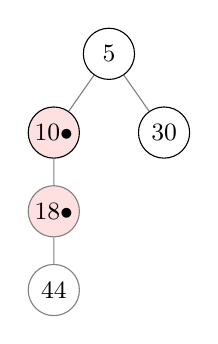
\begin{tikzpicture}[
  every node/.style={circle,draw,minimum size=6.5mm,inner sep=1pt,font=\small},
  level distance=10mm, sibling distance=14mm,
  edge from parent/.style={draw,gray}]
  \node {5}
    child {node[fill=red!12] {10$\bullet$}
      child {node[fill=red!12] {18$\bullet$}
        child {node {44}}}}
    child {node {30}};
\end{tikzpicture}
\end{center}

Both $10$ and $18$ are marked --- each has already lost one child in the past. Now
we call decrease-key on $44$, lowering it to $2$.

\begin{enumerate}
  \item $44 \to 2$. Its parent is $18$, and $2 < 18$, so heap order is violated.
        \textsc{Cut} $2$ from $18$: node $2$ flies up to the root list, unmarked.
        Now $18$ has lost a child.
  \item \textsc{Cascading-Cut}($18$): $18$ is already marked, so we cut \emph{it}
        too. Node $18$ flies up to the root list (still carrying nothing now, since
        $44$/$2$ already left), unmarked. Now $10$ has lost a child.
  \item \textsc{Cascading-Cut}($10$): $10$ is already marked, so we cut \emph{it}
        too. Node $10$ flies up to the root list, unmarked. Now $5$ has lost a
        child.
  \item \textsc{Cascading-Cut}($5$): $5$ is a root (no parent), so we stop.
\end{enumerate}

The single decrease-key triggered a chain of three cuts. Figure~\ref{ch20:fig-cascading-cuts}
shows the before-and-after. The root list grew by three trees ($2$, $18$, $10$),
each now unmarked. One decrease-key, several cuts --- and yet we are about to prove
that decrease-key still costs only $O(1)$ \emph{amortized}. The reason is that all
those cuts were ``pre-paid'' by the marks.

\begin{figure}[htbp]
\centering
\begin{tikzpicture}[font=\small, scale=0.95, transform shape]
  % Panel (a): Before decrease-key
  \begin{scope}
    \node[font=\footnotesize\scshape, text=gray!70!black] at (0, 1.2) {(a) Before: decreasing $44 \to 2$};
    \node[circle, draw=black, fill=white, thick, minimum size=7mm] (n5) at (0,0) {5};
    \node[circle, draw=trapred, fill=red!15, very thick, minimum size=7mm] (n10) at (-0.8,-1.1) {10$^\bullet$};
    \node[circle, draw=black, fill=white, thick, minimum size=7mm] (n30) at (0.8,-1.1) {30};
    \node[circle, draw=trapred, fill=red!15, very thick, minimum size=7mm] (n18) at (-0.8,-2.2) {18$^\bullet$};
    \node[circle, draw=quotientorange, fill=quotientorange!25, very thick, minimum size=7mm] (n44) at (-0.8,-3.3) {44};

    \draw[thick] (n5) -- (n10); \draw[thick] (n5) -- (n30);
    \draw[thick] (n10) -- (n18);
    \draw[thick] (n18) -- (n44);

    \node[font=\tiny, text=trapred!90!black, left=2pt of n18] {marked};
    \node[font=\tiny, text=trapred!90!black, left=2pt of n10] {marked};
  \end{scope}

  % Transition Arrow
  \draw[-{Latex[length=3mm]}, very thick, trapred] (1.8, -1.5) -- 
    node[above, font=\tiny, text=trapred, align=center] {Cascade: 3 cuts!\\$44, 18, 10$ cut\\marks cleared} (4.2, -1.5);

  % Panel (b): After cascading cuts
  \begin{scope}[xshift=5.8cm]
    \node[font=\footnotesize\scshape, text=gray!70!black] at (1.8, 1.2) {(b) After: nodes propelled into root list};
    
    % Root list nodes
    \node[circle, draw=black, fill=white, thick, minimum size=7mm] (r5) at (0, 0) {5};
    \node[circle, draw=black, fill=white, thick, minimum size=7mm] (r30) at (0, -1.1) {30};
    \draw[thick] (r5) -- (r30);

    \node[circle, draw=black, fill=white, thick, minimum size=7mm] (r10) at (1.4, 0) {10};
    \node[circle, draw=black, fill=white, thick, minimum size=7mm] (r18) at (2.6, 0) {18};
    \node[circle, draw=targetgreen, fill=targetgreen!25, very thick, minimum size=7mm] (r2) at (3.8, 0) {2$^*$};

    \draw[<->, dashed, thick, sourceblue] (r5) -- (r10);
    \draw[<->, dashed, thick, sourceblue] (r10) -- (r18);
    \draw[<->, dashed, thick, sourceblue] (r18) -- (r2);

    \node[font=\tiny, text=targetgreen!90!black, above=2pt of r2] {new min};
    \node[font=\tiny, text=gray!70!black] at (2.0, -1.5) {All $3$ cleared their mark;};
    \node[font=\tiny, text=gray!70!black] at (2.0, -1.8) {Root 5 was unmarked, stays valid.};
  \end{scope}
\end{tikzpicture}
\caption{A cascading cut during \textsc{Decrease-Key}. Key $44$ is decreased to $2 < 18$, prompting an initial cut. Because parent $18$ and grandparent $10$ were already marked (each having previously lost a child), the loss triggers a chain reaction of cascading cuts. Both $18$ and $10$ are severed, stripped of their marks, and placed in the root list. The potential $\Phi = t + 2m$ drops by $\Delta \Phi \le -1$, paying for the cascade.}
\label{ch20:fig-cascading-cuts}
\label{ch20:cascade}
\end{figure}

\begin{walkbox}
Before you read the analysis, go for a walk with this puzzle. A decrease-key can,
in the worst single case, trigger a long cascade of cuts --- so its \emph{actual}
cost is not constant at all; it can be $\Theta(\log n)$ for one unlucky call. Yet
we are going to call the cost $O(1)$ amortized. Where could the ``saved up'' money
for a long cascade have come from? Hint: think about what had to happen, earlier
and cheaply, for all those nodes to become marked in the first place.
\end{walkbox}

\section{The amortized analysis}

This is the heart of the chapter. Everything so far was setup; now we make the
$O(1)$ and $O(\log n)$ claims precise using the \emph{potential method} you met in
Chapter~17. If that method is hazy, here is the one-line
reminder: we invent a ``bank balance'' $\Phi$ that depends only on the current
state, and we define the \emph{amortized} cost of an operation as its real cost
plus the change in the balance, $\hat{c} = c + \Delta\Phi$. If the balance never
goes below its starting value, the total amortized cost is a valid upper bound on
the total real cost.

\subsection{Choosing the potential}

We need a potential that goes \emph{up} cheaply when we are being lazy (so future
cleanups are pre-funded), and goes \emph{down} when we finally clean up (refunding
the cleanup). Two things accumulate during laziness: extra trees in the root list,
and marked nodes. So we charge for both.

\begin{formalbox}
For a Fibonacci heap $H$, let $t(H)$ be the number of trees in the root list and
$m(H)$ the number of marked nodes. Define the potential
\[
  \Phi(H) \;=\; t(H) \;+\; 2\,m(H).
\]
An empty heap has $\Phi = 0$, and $\Phi$ is never negative, so amortized costs sum
to an upper bound on real costs.
\end{formalbox}

Why $2m$ rather than simply $m$? Because a cascading cut does two jobs at once when it
fires: it removes a mark \emph{and} it creates a new tree. We need each mark to
have stored enough to pay for both. Two units per mark is exactly the right
deposit, as the decrease-key analysis will show.

\subsection{Insert, minimum, union}

\textbf{Insert.} Real cost $O(1)$. It adds one tree, so $\Delta t = +1$; marks
unchanged. Thus $\Delta\Phi = +1$ and the amortized cost is $O(1) + 1 = O(1)$.

\textbf{Minimum and Union.} Neither changes $t$ or $m$ in any meaningful way
(union just concatenates root lists; the tree count of the combined heap equals the
sum). $\Delta\Phi = 0$, amortized cost $O(1)$.

\subsection{Extract-min}

Let $D(n)$ be the maximum possible degree of any node in an $n$-node Fibonacci
heap. We will prove in Section~\ref{ch20:why-fibonacci} that $D(n) = O(\log n)$;
take it on loan for now.

\emph{Real cost.} Step 1 promotes the children of the minimum --- at most $D(n)$ of
them --- to roots: $O(D(n))$. Step 2, consolidation, walks the root list. After
step 1 the root list has at most $D(n) + t(H) - 1$ trees (the original trees, minus
the extracted root, plus its promoted children). Each \textsc{Link} reduces the
number of roots by one and costs $O(1)$, and the final scan to rebuild the root
list and find the new min touches each surviving slot once, of which there are at
most $D(n)+1$. So the real cost is $O(D(n) + t(H))$.

\emph{Potential change.} Before consolidation, $t(H)$ trees; afterward, at most
$D(n)+1$ trees (one per distinct degree). Marks only ever decrease here. So
\[
  \Delta\Phi \;\le\; \big[(D(n)+1) + 2m(H)\big] - \big[t(H) + 2m(H)\big]
            \;=\; D(n) + 1 - t(H).
\]

\emph{Amortized cost.}
\[
  \hat{c} = O(D(n) + t(H)) + \big(D(n) + 1 - t(H)\big)
          = O(D(n)) = O(\log n).
\]
The $t(H)$ terms cancel: the more trees there were to clean up (high real cost),
the more potential we release (big refund). That cancellation is the whole point of
the potential. Extract-min is $O(\log n)$ amortized.

\subsection{Decrease-key}
\label{ch20:decrease-key-analysis}

Now let us see how the stored marks pay for cascading cuts. Suppose a single decrease-key triggers $c$ cuts in total
(one direct cut, then $c-1$ cascading cuts).

\emph{Real cost.} The direct cut plus $c-1$ cascading cuts, each $O(1)$: total
$O(c)$.

\emph{Potential change.} Track the two pieces of $\Phi = t + 2m$:
\begin{itemize}
  \item \textbf{Trees.} Every one of the $c$ cuts moves a node to the root list, so
        $t$ increases by $c$. That is $\Delta t = +c$.
  \item \textbf{Marks.} Each of the $c-1$ cascading cuts was performed \emph{on a
        marked node}, and \textsc{Cut} clears that mark: that removes $c-1$ marks.
        The cascade stops at one node that was unmarked and now becomes marked:
        that adds back at most $1$ mark. Net: $m$ changes by at most
        $-(c-1) + 1 = -(c-2) = 2 - c$. So $2\,\Delta m \le 2(2-c) = 4 - 2c$.
\end{itemize}
Adding up,
\[
  \Delta\Phi \;\le\; c + (4 - 2c) \;=\; 4 - c.
\]

\emph{Amortized cost.}
\[
  \hat{c} \;=\; O(c) + (4 - c).
\]
Write the $O(c)$ as $a\,c$ for some constant $a$ by choosing the potential
units large enough that each cut's real work is at most one unit of potential
($\hat c = c + (4-c) = 4 = O(1)$). The $c$ terms cancel exactly: the real cost of a
long cascade is paid, unit for unit, by the marks that the cascade releases. What
remains is a constant.

\begin{focusbox}
\textbf{This is the payoff.} A single decrease-key might really do
$\Theta(\log n)$ work via a long cascade. But every cut in that cascade spends a
mark that was \emph{deposited earlier}, one cheap unit at a time, by previous
decrease-keys. The bank balance $\Phi = t + 2m$ exactly funds the cascade. So no
matter how the work clusters, decrease-key is $O(1)$ amortized. The factor of $2$
on $m$ is what lets each mark pay for both the cut's work and the new tree the cut
creates.
\end{focusbox}

\subsection{Delete}

To delete an arbitrary node $x$: decrease its key to $-\infty$ (which floats it up
to become the minimum), then extract-min. Amortized cost
$O(1) + O(\log n) = O(\log n)$.

\begin{complexitybox}
With potential $\Phi = t + 2m$, every bound is amortized except where noted:
\[
\begin{array}{lll}
\textsc{Make-Heap} & O(1) & \text{worst case}\\
\textsc{Minimum} & O(1) & \text{worst case}\\
\textsc{Insert} & O(1) & \\
\textsc{Union} & O(1) & \text{worst case}\\
\textsc{Extract-Min} & O(\log n) & \\
\textsc{Decrease-Key} & O(1) & \\
\textsc{Delete} & O(\log n) & \\
\end{array}
\]
Here $n$ is the number of nodes and $D(n) = O(\log n)$ is the maximum degree.
\end{complexitybox}

\section{Why ``Fibonacci''? The degree bound}
\label{ch20:why-fibonacci}

We have leaned twice on the claim $D(n) = O(\log n)$: a node with $n$ descendants
cannot have huge degree. Now we earn it, and the proof is where the data structure
gets its name.

\subsection{What the mark rule guarantees}

The mark-and-cascade rule has a precise structural consequence. Consider any node
$x$ and list its current children in the order they were linked to $x$:
$y_1, y_2, \ldots, y_k$, where $y_i$ was the $i$-th child attached.

\begin{lemma}[The size each child must carry]
\label{ch20:degree-lemma}
With the children ordered by time of attachment, the $i$-th child $y_i$ has degree
at least $i - 2$ (for $i \ge 2$); and $y_1$ has degree at least $0$.
\end{lemma}

\begin{intuitionbox}
Here is why. When $y_i$ was linked to $x$, that link happened during a
consolidation between two roots of \emph{equal} degree. At that moment $x$ already
had children $y_1,\ldots,y_{i-1}$, so $x$'s degree was $i-1$, and therefore $y_i$'s
degree was also $i-1$. Since then, $y_i$ is allowed to lose \emph{at most one}
child before it would have been cut away from $x$ entirely (the mark rule!). So
$y_i$'s degree now is at least $(i-1) - 1 = i - 2$. That single subtracted child is
exactly what the mark bit is rationing.
\end{intuitionbox}

\subsection{Fibonacci numbers fall out}

Let $s_d$ be the \emph{minimum} possible number of nodes in a subtree whose root
has degree $d$. We want a lower bound on $s_d$. The root itself is one node. Its
children, by Lemma~\ref{ch20:degree-lemma}, have degrees at least
$0, 0, 1, 2, \ldots, d-2$. So the smallest such subtree satisfies
\[
  s_d \;\ge\; 1 + 1 + \sum_{i=2}^{d} s_{i-2}
       \;=\; 2 + \sum_{j=0}^{d-2} s_j,
\]
with $s_0 = 1$ and $s_1 = 2$. If you have seen the Fibonacci recurrence
$F_{k} = F_{k-1} + F_{k-2}$, the next line will feel familiar. One can show by
induction that
\[
  s_d \;\ge\; F_{d+2},
\]
where $F_k$ are the Fibonacci numbers ($F_0=0, F_1=1, F_2=1, F_3=2,\ldots$). The
sum-of-all-previous form above collapses, via the identity
$F_{d+2} = 1 + \sum_{i=0}^{d} F_i$, into the familiar two-term recurrence. \emph{This
is the moment the data structure earns its name:} the worst-case bushiness of its
trees is governed by exactly the Fibonacci sequence.

Figure~\ref{ch20:mintrees} draws the smallest possible trees of each degree and
counts their nodes; the counts are exactly $s_0,s_1,s_2,s_3 = 1,2,3,5$ --- the
Fibonacci numbers $F_2,F_3,F_4,F_5$ marching by.

\begin{figure}[H]
\centering
\begin{tikzpicture}[
  every node/.style={circle,draw,minimum size=5.5mm,inner sep=1pt,font=\footnotesize,fill=structurepurple!12},
  level distance=8mm, sibling distance=9mm,
  edge from parent/.style={draw,gray}]
  % degree 0: 1 node
  \begin{scope}[xshift=0cm]
    \node {$\bullet$};
    \node[draw=none,fill=none,font=\footnotesize] at (0,-1.0) {$d{=}0$};
    \node[draw=none,fill=none,font=\footnotesize] at (0,-1.5) {$s_0{=}1$};
  \end{scope}
  % degree 1: 2 nodes
  \begin{scope}[xshift=1.8cm]
    \node {$\bullet$} child {node {$\bullet$}};
    \node[draw=none,fill=none,font=\footnotesize] at (0,-1.4) {$d{=}1$};
    \node[draw=none,fill=none,font=\footnotesize] at (0,-1.9) {$s_1{=}2$};
  \end{scope}
  % degree 2: 3 nodes (children of degrees 0,0)
  \begin{scope}[xshift=3.9cm]
    \node {$\bullet$}
      child {node {$\bullet$}}
      child {node {$\bullet$}};
    \node[draw=none,fill=none,font=\footnotesize] at (0,-2.0) {$d{=}2,\ s_2{=}3$};
  \end{scope}
  % degree 3: 5 nodes, children of degrees 0,0,1
  \begin{scope}[xshift=7.0cm]
    \node {$\bullet$}
      child {node {$\bullet$}}
      child {node {$\bullet$}}
      child {node {$\bullet$} child {node {$\bullet$}}};
    \node[draw=none,fill=none,font=\footnotesize] at (0,-2.7) {$d{=}3,\ s_3{=}5$};
  \end{scope}
\end{tikzpicture}
\caption{The leanest trees a degree-$d$ root can be reduced to under the mark rule,
for $d=0,1,2,3$. Their node counts $1,2,3,5$ are the Fibonacci numbers
$F_{d+2}$. The children are forced to have degrees $0,0,1,\ldots,d-2$, and feeding
those minimal sizes into $s_d \ge 2 + \sum_{j=0}^{d-2} s_j$ makes the counts
satisfy $s_d = s_{d-1} + s_{d-2}$ --- the Fibonacci recurrence.}
\label{ch20:mintrees}
\end{figure}

\begin{formalbox}
\textbf{The size--degree bound.} A node of degree $d$ in a Fibonacci heap has at
least $F_{d+2} \ge \phi^d$ descendants (including itself), where
$\phi = \tfrac{1+\sqrt5}{2} \approx 1.618$ is the golden ratio. Consequently, if a
heap has $n$ nodes, the maximum possible degree is
\[
  D(n) \;\le\; \log_\phi n \;=\; O(\log n).
\]
\end{formalbox}

\begin{historybox}
Fibonacci heaps were invented by Michael L.~Fredman and Robert E.~Tarjan in 1984 (published in 1987). Their explicit motivation was breaking the asymptotic bottleneck of Dijkstra's single-source shortest-path algorithm and Prim's minimum-spanning-tree algorithm. On a dense graph with $V$ vertices and $E \approx V^2$ edges, binary heaps spend $O(E\log V)$ total time, with almost all time spent repeatedly lowering priority keys during edge relaxation (updating a neighbor's tentative distance when a newly explored edge offers a shorter route). Fredman and Tarjan designed a priority queue that reduced \lstinline|decrease-key| from $O(\log n)$ to $O(1)$ amortized, achieving the landmark $O(V\log V + E)$ running time.

The natural temptation when making \lstinline|decrease-key| fast is to cut any violating child and immediately move it to the root list. This naive cut is $O(1)$ worst-case, but it rapidly ruins the heap: over thousands of cuts, a parent can be stripped of nearly all its children, degenerating trees into tall, spindly chains. Without a bound on tree bushiness, a node of degree $d$ might contain only $O(d)$ descendants rather than exponential descendants, blowing up the degree bound $D(n)$ to $\Theta(n)$ and causing \lstinline|extract-min| consolidation to degrade to catastrophic $\Theta(n)$ time. Fredman and Tarjan solved this with the mark bit: allowing a node to lose at most one child before being evicted itself guarantees that tree sizes grow as $s_d \ge F_{d+2} \ge \phi^d$, maintaining $D(n) \le \log_\phi n = O(\log n)$.

Fibonacci heaps became the theoretical gold standard for priority queues, delivering $O(V\log V + E)$ shortest paths and minimum spanning trees, along with $O(1)$ amortized insertion and merging. Yet this carries an honest trade-off: high constant factors and pointer bloat. Each node requires four pointers (parent, left sibling, right sibling, child), an integer degree, and a boolean mark (amounting to dozens of bytes per element). On modern CPUs with deep cache hierarchies, the pointer-chasing overhead of Fibonacci heaps makes them slower in practice than 4-ary binary heaps or self-adjusting pairing heaps for all but astronomical graph sizes. Designing a priority queue that achieves $O(1)$ decrease-key with strict worst-case bounds, minimal pointer overhead, and cache locality remains an active open pursuit in data structures.
\end{historybox}

\begin{aestheticbox}
The golden ratio $\phi$ is not decoration here; it does real work. Because
each node of degree $d$ is forced to hide at least $\phi^d$ descendants, degree
grows only \emph{logarithmically} in the number of nodes, which is exactly what
makes consolidation's tidy-up cost $O(\log n)$. Loosen the mark rule and the base
of that logarithm degrades; tighten it and you would pay more per decrease-key.
Fredman and Tarjan found the balance point, and the golden ratio is what falls
out of it.
\end{aestheticbox}

\section{Putting it back in context: Dijkstra and Prim}

Now we can close the loop we opened in Section~\ref{ch20:problem}. Recall Dijkstra
on a graph with
$V$ vertices and $E$ edges performs:

\begin{itemize}
  \item one \lstinline|insert| per vertex: $V$ inserts, $O(V)$ amortized total;
  \item one \lstinline|extract-min| per vertex: $V$ extracts, $O(V \log V)$
        amortized total;
  \item up to one \lstinline|decrease-key| per edge during relaxation: $E$
        decrease-keys, $O(E)$ amortized total.
\end{itemize}

Add them: $O(V \log V + E)$. Compare with the binary-heap implementation's
$O((V+E)\log V) = O(E\log V)$ on a connected graph. On a \emph{dense} graph where
$E = \Theta(V^2)$, the Fibonacci version does $O(V^2)$ work for relaxation instead
of $O(V^2\log V)$ --- a clean $\log V$ saved, exactly where the algorithm spends
most of its time.

\begin{aestheticbox}
A caveat worth its own paragraph, because textbooks sometimes oversell Fibonacci
heaps. The constant factors and pointer-chasing overhead are real, and on the
\emph{sparse} graphs that dominate practice ($E = O(V)$), a plain binary heap or a
$d$-ary heap is usually faster on the wall clock despite its worse asymptotics. So
in everyday code, Fibonacci heaps are rare. Their importance is twofold: they prove
what is theoretically \emph{possible} (the best known asymptotic bound for Dijkstra
in the comparison model for a long time), and the amortized-analysis techniques
they teach --- lazy structure plus a potential that pre-funds cleanup --- recur all
over algorithm design. You are learning a way of \emph{thinking} as much as a
specific gadget.
\end{aestheticbox}

\section{Summary}

\begin{focusbox}
\begin{itemize}
  \item A Fibonacci heap is a \emph{forest} of heap-ordered trees with a pointer to
        the minimum root. It is deliberately lazy.
  \item \lstinline|insert| and \lstinline|union| just splice into the root list:
        $O(1)$. \lstinline|minimum| reads a pointer: $O(1)$.
  \item \lstinline|extract-min| is the one cleanup: promote the min's children,
        then \emph{consolidate} so that no two roots share a degree. This is
        $O(\log n)$ amortized.
  \item \lstinline|decrease-key| cuts a violating node up to the root list and uses
        the \emph{mark bit} to bound how lopsided trees can get, via \emph{cascading
        cuts}. It is $O(1)$ amortized.
  \item The potential $\Phi = t(H) + 2m(H)$ (trees plus twice the marked nodes)
        funds the cleanups: long cascades are paid for by marks deposited earlier.
  \item The mark rule forces a degree-$d$ node to hide at least $F_{d+2}\ge\phi^d$
        descendants, so $D(n) = O(\log n)$ --- which is where ``Fibonacci'' comes
        from.
  \item Net effect: Dijkstra and Prim drop to $O(V\log V + E)$, a real win on dense
        graphs.
\end{itemize}
\end{focusbox}

Fibonacci heaps push comparison-based priority queues to their theoretical limits:
as long as keys can only be compared pairwise, an $\Omega(\log n)$ lower bound governs
sorting and priority queue extractions. To beat this bound, we must change the rules of
the game.

What if our keys are not arbitrary opaque objects, but integers drawn from a bounded
universe $\{0, 1, \dots, u-1\}$? In \textbf{Chapter~21 (van Emde Boas Trees)}, we break
through the comparison barrier entirely. By decomposing an integer universe recursively
into clusters of size $\sqrt{u}$, van Emde Boas trees achieve $O(\log \log u)$ time for
search, predecessor, successor, minimum, maximum, insert, and delete --- a running time
so fast that even for a universe of four billion 32-bit integers, every operation takes
fewer than six recursive steps.

\section*{Exercises}
\addcontentsline{toc}{section}{Exercises}

\begin{exercise}[Warmup: insert only]
Start from an empty Fibonacci heap and insert the keys $8, 3, 11, 1, 6$ in order.
Draw the heap after each insert, showing the root list and the $\mathit{min}$
pointer. How many trees are in the root list at the end, and what is $\Phi$?
\end{exercise}

\begin{exercise}[Consolidation by hand]
Continue from the previous exercise and call \textsc{Extract-Min} once. Carry out
\textsc{Consolidate} using a degree array, writing down the contents of $A$ after
each root is processed. Draw the resulting forest and give the new $\mathit{min}$.
\end{exercise}

\begin{exercise}[Cascading cut]
Build (or accept as given) a tree rooted at $4$ with a chain of children
$4 \to 9 \to 15 \to 26 \to 40$, where $9$, $15$, and $26$ are all marked. Call
decrease-key on $40$, lowering it to $1$. List every \textsc{Cut} and
\textsc{Cascading-Cut} that fires, and state how many trees the root list gains.
\end{exercise}

\begin{exercise}[Potential bookkeeping]
For the decrease-key in the previous exercise, compute the real cost (count the
cuts), the change $\Delta\Phi$ in the potential $\Phi = t + 2m$, and the amortized
cost $\hat c = c + \Delta\Phi$. Confirm it is a constant.
\end{exercise}

\begin{exercise}[Why twice the marks?]
Redo the decrease-key amortized analysis of
Section~\ref{ch20:decrease-key-analysis} using the potential
$\Phi' = t(H) + m(H)$ (only \emph{one} unit per mark). Show that the $c$ terms no
longer cancel, and identify the exact step that breaks. Explain in one sentence why
the coefficient $2$ is necessary.
\end{exercise}

\begin{exercise}[Degree bound, small cases]
Using $s_0 = 1$, $s_1 = 2$, and $s_d \ge 2 + \sum_{j=0}^{d-2} s_j$, compute lower
bounds $s_2, s_3, s_4, s_5$. Compare each to the Fibonacci number $F_{d+2}$ and to
$\phi^d$. At what degree does a node first guarantee at least $20$ descendants?
\end{exercise}

\begin{exercise}[Worst-case versus amortized]
Construct a sequence of operations on a Fibonacci heap in which a \emph{single}
decrease-key really performs $\Theta(\log n)$ cuts. (Hint: you must first arrange a
long chain of marked nodes; describe how a sequence of decrease-keys and
extract-mins can set that up.) Explain why this does not contradict the $O(1)$
amortized bound.
\end{exercise}

\begin{exercise}[Dijkstra accounting]
On a graph with $V = 1000$ vertices and $E = 400{,}000$ edges, write the total
amortized cost of Dijkstra using (a) a binary heap and (b) a Fibonacci heap, as
expressions in $V$ and $E$. Which wins asymptotically here, and roughly by what
factor in the relaxation term? Would your answer change for a sparse graph with
$E = 3V$?
\end{exercise}

\begin{exercise}[Mergeable advantage]
Describe a scenario --- a concrete algorithm or workload --- where the $O(1)$
\textsc{Union} of a Fibonacci heap is the deciding advantage over a binary heap.
Estimate the asymptotic saving for $k$ merges of heaps with $n$ total elements.
\end{exercise}

\begin{exercise}[Challenge: no decrease-key?]
Some applications never call decrease-key (for example, certain event-simulation
queues). In that restricted setting, the mark bit and cascading cuts are never
exercised. Argue what the amortized bounds become, and explain why, in this
decrease-key-free world, a simpler ``lazy binomial heap'' suffices and the
Fibonacci machinery buys you nothing.
\end{exercise}
